\section{Multi-band Adaptation---Opportunity and Algorithms}
\label{sec:model}

In this section, we will investigate optimal bands selection in multi-band channels. 

\subsection{Problem Formulation of Multiband selection}
\label{subsec:problem}
Assume there are K bands, the throughput vector across all bands as $T_{pt}=[r_1,r_2,...r_k]$, which depends on received signal power, noise, interference and so on. Comparing with traditional frequency-selective channels, in multi-band session, path loss is an important factor for received signal power in different channels. 
Path loss increases with distance from the base and related to the wavelength the decibel path loss can be presented as:\cite{rappaport}

\begin{align}
\label{euqation:path loss}
P_{R}=\frac{P_TG_TG_R\lambda}{d^\alpha(4\pi)^2}
\end{align}

where ,$P_R$ is the received signal of receiver node, $P_T$ is the transmitting power, $G_T,G_R$ represent the antennas gain at transmitting and receive sides,
$\lambda$ is the wavelength, $\alpha$ is the path loss exponent related to the environment. 

Signal level is widely used to represent the dynamic channel state  \cite{rahul2009frequency}. 
From \ref{equation:pass loss} we could see the revceived signal is related to the wavelength, and the wavelength $\lambda$ can be represented as $\lambda=frac{C}{Frequency}$. So multi-band devices could have performance improvement because of the connection between frequency and received signal.


%\subsection{Dynamic and Correlation Info}

%1,How to evaluate channel
%2,SNR
Many hardware manufactures already perform the SNR/Received signal strength detection character as part of the hardware specification \cite{edalat2006measured}. 
The RSSI(Received Signal Strength Indication) is consider as an important factor for throughput performance estimate.\cite{laneman2000energy,laneman2001efficient}. 

%In this paper, signal level is also an important factor for the performance database.
%3,Loss based
Furthermore, except RSSI, other factors also represent the channel state. Channel Statistics information is used by lots of adaptation algorithms in previous research.
FARA tracks the the number of active clients, then update the next-hop table for transmission\cite{rahul2009frequency}.
The statistics of collisions and link errors also could be considered as channel qualification factors \cite{pang2005rate}.
Our work also investigate the influence of activity in in-field channel.
%4,The definitation of the activity level

The \emph{Activity Level} present the utility level of the channel
which is defined as a statistics of band occupied time ratio. Through the temporal correlation parameter, the prediction of the performance could fits in-field system channel state estimation better than only consider the dynamic channel state.
In our work, the definition of activity can be represented by:
%Non 802.11 interference
For the white band which is primarily used by TV and cellphones, the activity level could be defined as:
\begin{align}
\label{equation:non802 Activity Level}
Activity\,Level = \sum{\frac{Interferencei\ Active\ Time}{Duration}}
\end{align}
%802.11 interference
For 802.11 standard band, 2.4GHz and 5GHz, the activity level is defined as:
\begin{align}
\label{equation:802 Activity Level}
Activity\,Level = \sum{\frac{(All\, Packets)-(Connection\, Packets)}{Rate*Duration}}
\end{align}

All packets is the amount of packets received in one band during a time slot.
The connection packets is the amount of packets received by particular transmitter and receiver pair. 
The length and transmitting rate of each packet are collected to calculate the activity level.
The \emph{Activity Level} is a \emph{ratio} that occupied by the interference transmitter during a time slot. 
%We assume all the nodes have a common rate or could be averaged to a transmission rate. 
%It represents the free time ratio can be used by the particular transmitter and receiver transmission. 
%The transmission of interference nodes has correlation between continuous periods, especially the beacon packets. So the previous channel state can be used as a parameter for estimating current channel states.

%5,How we use these information
%Fixme{Figure}


%Different variations of we consider include: 
%(\emph{i}) We map the context information to find the maximize throughput across the bands in vehicular channel model.
%(\emph{ii}) We verify our protocol through in-field experiments data collecting in vehicles. 
%The corresponding maximal throughput,$G^*$, serves as an upper bound to the performance that can be achieved by multi-band adaptation. 
%This upper bound is computed from the training data on emulator employing  as the performance in ideal channel and all transmission time is free to use for the focused transmission pair.
%
%



%In an ideal channel, if the received signal is the same among all the bands, the performance should be the same. It is a reasonable assumption verified by experiments on the emulator. The performance across different bands in different received signal shows as: {fixme insert throughput vs rssi in bypass}
As we discussed, path loss varies in different channels, providing opportunity for maximizing throughput through band selection. However, for in-field application, due to environment, traffic and interference, it is difficult to quantitative analysis path loss. 
To implement the multi-band selection, we borrow the context-aware idea to evaluate channel state instead of theoretic analysis of path loss and other parameters. 

%We focus on a point to point communication pair system. 
%From the equation, the antennas gain $G_T,G_R$ is fixed for a communication system, and the distance from the transmitter to the receiver is fixed.
%And also due to limitations imposed by the FCC, the transmit power $P_T$ of an access point is restricted. 
%So in such a wireless system, the $P_R$ of the receive node is determined by two parameters. One is the path loss exponent $\alpha$, another is the wavelength of the operating channel. 
%Our research focus on the situation the radios in different bands work on the same node, they operate in the same environment, so the path loss exponent for different bands should be the same. 
%The path loss exponent in an environment usually be estimated by measuring the received power and distance between the transmit and receive nodes. According to these measurements, a fitting exponent curve can be used to get the path loss exponent. fixme insert rx-power and distance graph 



%Then, for a multi-band/multi-radio system can work on different bands, wavelength become the most important factor influence the received power.
%In an ideal channel, if the received signal is the same among all the bands, the performance should be the same. It is a reasonable assumption verified by experiments on the channel emulator. The performance across different bands in different received signal shows as: {fixme insert throughput vs rssi in bypass}

%In the limited access range, the path loss of different bands are varying according to their wavelength. 
%The difference of received signal makes the performance vary in different bands. Then, for a particular environment, there is room to improve the performance in switching band.


%Another potential room  for wireless communication performance improvement is the utility level of a channel. Most of the wifi devices are working in 2.4GHz and 5GHz as 802.11 standard. Other interference signals, such as TV, GSM signals are shown in other bands. These interference signals, both 802.11 signals and other interference signals, are discontinuous. 
%For a multi-band communication, we treat these signals as primary users, try to find the spectrum opportunity and imprvoe the performance.

%Our method is to employ accumulate information in a time slot to quantify the channel state. The difference in crowd level of wireless channel also provide room for performance improvement in switching band.  
%In this section, we exploit channel dynamic and accumulate information in contextual data and develop band adaptation frame for dynamic environments.Through the proposed framework, we improve the throughput of a pair of multi-radio nodes according the given context. While in this paper we focus on the application to band adaptation to show gains, the framwork has other possible applications to transmission parameter adaptation based on context information. 


%room for improvement
%Spectrum sensing is the fundamental problem of cognitive radio and has reborn as a very active research area in recent years despite its long history\cite{zeng2010review}.
%It can be classed as \emph{Energy Detector Based Sensing, Matched Filter Detection, Cyclostationary Detection, Wavelet-based Detection, etc.} \cite{zeng2010review,zhao2007survey}.


%Objective
This work is to improve the performance of point to point multi-bands system in pratical environments based on estimation of channel states according to stored information.
%It is also very important for our framework to detect the channel state.
%previous research no propagation, no map to throughput
%Most of the previous research of spectrum sensing focus on the theoretical computation of detection probability and false alarm probability without considering the difference of propagation across different bands \cite{zeng2010review,zhao2007survey,chen2008joint,hou2011spectrum}. 
%In pratice, there are other factors such as system loss which could not be theoretical analyzing make it hard to exploit these spectrum sensing algorithms.
%Moreover, these researches do not show any wireless performance information related to the spectrum sensing directly. 

%Protocol has been built

Some multi-channel adaptation and rate adaptation researches focus on \emph{Dynamic Channel State} as represented by \cite{cordeiro2007c,MOAR}:. 
which distinguish that the performance is related to the channel state, but only involve the dynamic information and do not consider the variation across wide bands. 
Furthermore, the embedded temporal correlation of the wireless channel also represent the channel state \cite{liuastra}. 
%The interference factor gradually changing process makes the statistics have an embedded temporal correlation. 
%This paper's work
A method to develop these work is to consider context-aware information which provide a way to resolve the problem with history information for spectrum sensing prediction \cite{yucek2009survey}.
\begin{align}
\label{euqation:performance estimation}
f(SNR,Context-Aware\, Info) \rightarrow Performance\, Estimation
\end{align}

In this paper, our work involve historical information for channel state evaluation which also represent channel characters including path loss of different bands.
The \emph{Context-Aware Info} has parameters related to the performance of wireless networks, such as velocity of nodes, the location, and previous activity of the channel, etc. 
We use different sub-sets of the Context-Aware information to design multiple algorithms for utility in various application fields. 


%A performance mapping from the spectrum sensing is introduced and evaluated by experiments.

\subsection{Algorithms}
\label{subsec:algorithms}

\emph{Context-Aware Information} provides a way for the optimum bands selection. However, it is usually difficult to directly get all the Context-Aware Information at a time.Therefore, we develop methods to search the optimal band for maximizing throughput. In the following, we describe the ideal performance based algorithm, machine learning algorithm, location based look up algorithm, region slitted machine learning algorithm.

When a wireless node gets in to a strange area, there is only RSSI, activity of channels can be collected by the device. Then, the node can only rely on ideal performance from manufacture or self test of the node. For this case, we have the \emph{Ideal Performance Based Algorithm}

\emph{Ideal Performance Based Algorithm}
\emph{Input:} Dynamic RSSI $r_i$, Channel Activity State $a_i$, Ideal Performance Data $ideal_i$ 
\emph{Output:} Optimal transmission band: $b^*$

\begin{enumerate}
\item Look up performance from $ideal_i$ based on $r_i$, get ideal throughput $Tpt_{ideal}$
\item Based on the activity state adjust the throughput $Tpt_e=Tpt_{ideal}(1-Activity Level)$
\item Repeat Step 1,2 to get the predict throughput in all available bands
\item Compare the predict throughput of all the bands, find the best $b^*$
\item Return $b^*$
\end{enumerate}

%First step is to do the spectrum sensing and gather information across different bands. 
%Second is to predict performance among all the bands based on the spectrum sensing information. 
%Fix to add more 
%For the white band whose first user is TV or cellphones, the activity level is defined as:
%\begin{align}
%\label{equation:non802 Activity Level}
%Activity\,Level = \sum{\frac{Interference Active Time}{Duration}}
%\end{align}
%%802.11 interference
%For 802.11 standard band, 2.4GHz and 5GHz, the activity level is defined as:
%\begin{align}
%\label{equation:802 Activity Level}
%Activity\,Level = \sum{\frac{(All\, Packets)-(Connection\, Packets)}{Rate*Duration}}
%\end{align}
%
In a familiar area, previous information collected in this area can be used for band selection. Machine learning algorithm, Location based algorithm, and Region split machine learning algorithm are tested in this case.

Machine learning is counted as an important new way in wireless communication \cite{haykin2005cognitive}. When user re-entry an area, the previous data can be trained by machine learning algorithm and tell the device which band may have the best performance.
The \emph{Machine Learning Algorithm} can lead to the optimum band selection through several steps:

\emph{Machine Learning Algorithm}
\emph{Input:} Dynamic RSSI $r_i$, Channel Activity State $a_i$, Trained Decision Tree $M_i$, Velocity $v_i$ 
\emph{Output:} Optimal transmission band: $b^*$

\begin{enumerate}
\item Input Dynamic RSSI $ideal_i$, Channel Activity State $a_i$, Velocity $v_i$ of all 4 bands and follow the Decision Tree $M_i$ to reach the performance of a band
\item Repeat 1 to get the predict throughput in all available bands
\item Compare the predict throughput of all the bands, find the best $b^*$
\item Return $b^*$
\end{enumerate}

\emph{Machine Learning Algorithm} can find the inner pattern of different parameters. However, the machine learning algorithm could not include context-aware information which is not related to the performance directly, such as the location information. Also, due to the limited computation resource on mobile devices, it is difficult to train the data on the device itself. 
However, the location information is pretty important for vehicle utility.
Therefore, the \emph{Location Based Look up Algorithm} is developed to consider the location based on the previous data collected. The algorithm is an iteration method to find the data near the location and look for the best performance across bands.



\emph{Location Based Look up Algorithm}
\emph{Input:} Location $G_i$, Dynamic RSSI $r_i$,Previous Collected Data $D_i$, Channel Activity State $a_i$, Velocity $v_i$ 
\emph{Output:} Optimal transmission band: $b^*$

\begin{enumerate}
\item Find data collected in a range near current location in stored previous data
\item If the data amount is less than a threshold, then increase the range and repeat 1
\item Group the select data to a n-dimension look up table
\item Input Dynamic RSSI $r_i$, velocity $v_i$ to the look up table find data points have similar parameters in a range
\item If the data amount is less than a threshold, then increase the parameter range and repeat 4
\item Statistic the data points, find the best band $b^*$ who has the most best performance in statistics
\item Return $b^*$
\end{enumerate}

The \emph{Location Based Look up Algorithm} provide a simple way to include location information for prediction. To employ the powerful tool machine learning with location information, data is divided into different regions based on the location and develop as \emph{Split Region Machine Learning Algorithm}

\emph{Split Region Machine Learning Algorithm}
\emph{Input:} Location $G_i$, Dynamic RSSI $r_i$, Channel Activity State $a_i$, Previous Collected Data $D_i$, Velocity $v_i$ 
\emph{Output:} Optimal transmission band: $b^*$

\begin{enumerate}
\item Split the  into N regions based on Location $G_i$ 
\item Processing the data in a region get the trained data $M_{n,i}$ 
\item Get the current location information of the node, find the current region 
\item Input Dynamic RSSI $ideal_i$, Channel Activity State $a_i$, Velocity $v_i$ of all 4 bands and follow the Decision Tree $M_{n,i}$ to reach the performance of a band
\item Repeat 4 to get the predict throughput in all available bands
\item Compare the predict throughput of all the bands, find the best $b^*$
\item Return $b^*$
\end{enumerate}


 

%The performance context-aware database is created on simulated channel. The input of the database includes channel type, velocity and SNR.
%Channel type indicates the propagation and fading characteristics between the transmitter and receiver. Many factors(e.g., multi-path, path loss, and shadowing) have a substantial influence on the characteristics of the channel type \cite{liuastra}. We use ITU channel types to generate the performance database, which are widely accepted as representative channel types for urban and suburban settings \cite{recommendation19971225}.


%The objective of this work is to demonstrate the improvements in performance by leveraging information of ideal channels to make band adapatation decisions. As noted before, the context information we consider is the channel type, measured received signal strength, received bytes, background noise and channel interference. The channel type indicates the propagation and fading characteristics between the transmitter and receiver. Many factors(e.g., multi-path, path loss, and shadowing) have a substantial influence on the characteristics of the channel type.FIXME{citation of Hui paper} However, in this paper, we assume the channel type to be a static channel type across all the wireless bands. We use the defination of ITU channels, which are widely accepted as representative channel types for urban dan suburban settings \cite{recommendation19971225}. Moreover, noise and interference gradually changes in the field. The gradually changing process makes it possible to seperate the noise, and even the interference from time varying experiments. 

%As far as we know, there is no work has done for such multi-band adaptation. 

%Problem formulation, equation style
%The optimization problem can be formulated as: in multi-radio/multi-bands system, given dynamic received signal level in part of the available bands, the activity level of all the bands, and context-aware information, which spectrum band should we choose. 




%We adapt the transmission band for each scenario based on the contextual information and the temporal correlation. 

%In this paper, we involve a factor \emph{Activity Level} to the framework. In this case, the multi-band adaptation can be simply represented as:


%\begin{align}
%f(Part\, Bands\, Signal\, Level,\nonumber \\
%All\,bands\, Activity\,Level, \nonumber \\
%Context-Aware\, Info)\nonumber \\
%\rightarrow max_{One Band}{Performance\, Estimation}
%\end{align}



%fixme, the figure should include the rssi estimate
%\begin{figure}
%\centering
%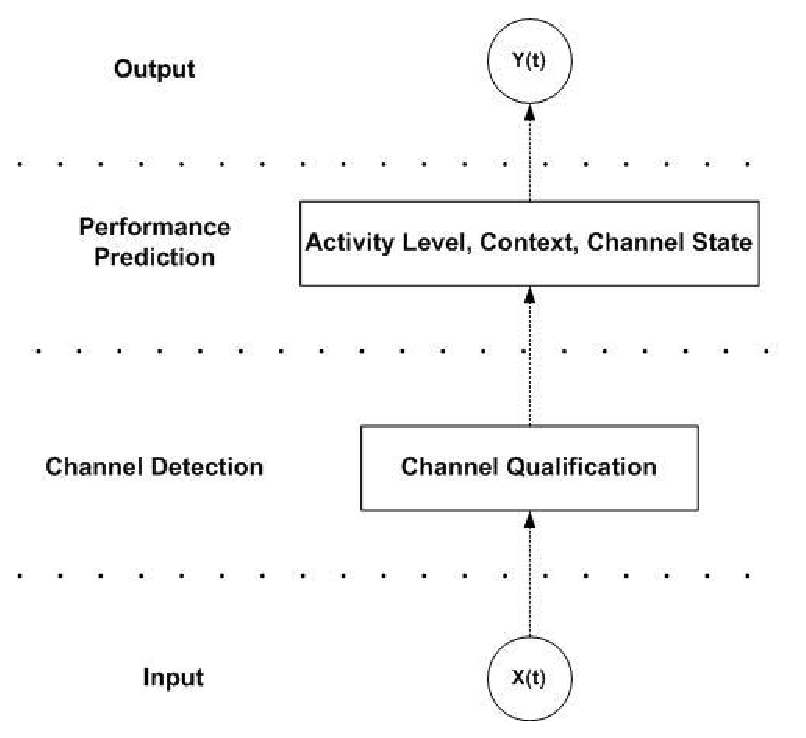
\includegraphics[width=85mm]{figure/multiband_framework}
%\caption{Multi-band framework.}
%\label{fig:multiframe}
%\end{figure}
%
%\subsection{Performance Prediction and Decision}
%
%The multi-band adaptation is receiver driven: the receiver
%estimates the channel state, predicts the optimal band and send the 
%prediction result back to the sender. The estimation process is 
%described as follows.
%
%Let $S = \{s_1, s_2, ..., s_N\}$ represent the set of bands 
%available for adaptation. In our experiments, we decide $S = \{450 MHz, 
%2.4 GHz, 5.8 GHz\}$ by considering commonly used wifi wireless bands.  
%Let $C = \{c_1, c_2, ...c_M\}$ represent the collected in-situ propagation 
%characteristics. We choose transmission delay $D$ and throughput $G_th$ as 
%the optimization metric in our experiments, which is modifiable upon the 
%interest of the users. 
%
%%The optimization problem is stated as follows: 
%Given a particular context $C$, select the optimal band $s^*$ that 
%maximizes the throughput, $G_{th}$ or minimize the delay $D$.
%Formally, the problems are posed as follows:
%\begin{eqnarray}
%\max_{s \in S}& G_{th}& = (1-\mbox{\it Activity Level})*R_{th} \label{eq:throughput_optimization} \\
%		\mbox{\it given} & & \mbox{\it Signal Strength}, \mbox{\it velocity}, \mbox{\it channel type} \nonumber
%		\end{eqnarray}
%
%\begin{eqnarray}
%\min_{s \in S}& D& = \frac1{\mbox{\it Activity Level}*R_{th}}\label{eq:delay_optimization} \\
%		\mbox{\it given} & & \mbox{\it Signal Strength}, \mbox{\it velocity}, \mbox{\it channel type} \nonumber
%		\end{eqnarray}
		
%$T_{ideal}$ is the throughput from the ideal channel conditions in emulator. 
%where Activity Level is a ratio as notified represent the time during one period occupied by other nodes. 

%The optimization problem is solved through several steps in our framework with the context-aware information.

%-up table has the relationship of SNR and throughput mapping generated from experiments in ideal channel states, in our case collecting the data on channel emulator.  





%%\subsection{Context-Aware Information}

%1,what is context info


%%Contexts, which defines various operating situations. Depending on a context, the wireless device changes its operational 
%%behavior in accordance with a defined profile, when a context parameter changes \cite{phillips2004wireless}. Context is a database include the knowledge the system stored or learned from the experiments or activities. Based on tons of measurement in different scenarios, a relationship between performance and system parameters can be created. 
%%For each piece of input parameters, the database can provide an output according to different algorithms.
%The collected contextual information is the input to the multi-band adaptaion model. In the ideal channel context information, for each given set of bands, SNR, the context table can represent ideal throughput for each bands. 

%2,how others use the info Fixme
%%In wireless communication, context-aware information is the experience of a transmit receiver pair. The performance of a system in the past can help transmute to find the optimal rate/band based on the parameter collected by the receiver. Such as in FARA algorithm, the receiver uses an SNR characterization table that lists the minimum SNR required for a particular combination of modulation and coding rate\cite{rahul2009frequency}. 
%3,how we use the info

%%In this paper, two context-aware database are exploited, one is the context-aware database for signal level across different bands, another one is the performance database. 
%%In the signal level context database, the input is signal level of one band, the output includes the signal level of other bands.
%%In the performance context information, we input the signal level, velocity and channel type to the database, then output the estimated throughput.  
%4,Difference
%%The output throughput is the middle state of our model to get the prediction of the performance, furthermore, adjustment will be put on these information. 


%%\begin{align}
%%f(Part\, Band\, Signal\, Level) \nonumber \\
%%\rightarrow Multi-band Signal Level
%%\end{align}

%%\begin{align}
%%f(Signal\, Level,Channel\, Type, Velocity, \nonumber \\ 
%%Context-Aware\, Info) \rightarrow Performance Estimation
%%\end{align}



%
%\subsection{Algorithm}
%\label{subsec:algorithm}
%We now describe three different approaches to do multiband adaptation.
%\subsubsection{Training on the emulated channel}
%We collect the training data on emulated channels with no interference from
%other wireless transmission. In this
%situation, each band can achieve its best throughput or delay performance.
%We record the SNR and idealized throughput or delay achieved. When the application
%is running in the field, the algorithm measures the activity level of each band 
%and predict the throughput or delay performance of each band.
%Based on~(\ref{eq:throughput_optimization}) 
%and~(\ref{eq:delay_optimization}), we select the optimal band with the best
%performance.
%
%%\begin{itemize}
%%\item \emph{Step 1} Create the signal level database for a location. The connection across different bands can be distinguished in this context-aware database.
%\item \emph{Step 1} Collect context data on emulator for different scenarios (Bands, Channel type, SNR, Velocity) to find the ideal state or the upper bound of the performance for one band.
%%\item \emph{Step 2} Collect context data on emulator for different scenarios (Bands, Channel type, SNR, Velocity) to create the performance database for the ideal state or the upper bound of the performance for each band.
%%\item \emph{Step 3} Detect the signal level in one band to qualify the wireless channel in all the bands dynamically, map the estimate signal level to the performance context-aware information in \emph{Step 2} finding the upper bound of for the current wireless channel state.  
%%\item \emph{Step 4} Compute the \emph{Activity Level} according to the statistic information, then re-calculate the estimate throughput including the \emph{Activity Level}.
%%\item \emph{Step 5} Compare the estimate throughput across all the bands and make the best choice among the available bands.
%%\end{itemize}

%%Through these steps, the transmitter and receiver pair updates the channel state and put the best band in working.

%\subsubsection{Location Agnostic In-Field Training}
%\label{subsubsec:noloca}
%In this case, we consider to collect the training data with in-field 
%experiments. The training data includes records of SNR, velocity, 
%activity-level and other in-situ propagation characteristics and the 
%optimal band in each of these cases. We apply machine learning techniques
%to learn the pattern in the relationship between the propagation characteristics
%and the potential performance in different bands. The pattern
%is formulated based on the training data as a mapping function, which
%can suggest the potential optimal band in practical application with 
%collected propagation characteristics. 
%
%%mobile: velocity, SNR, activity level->G/D, machine learning
%
%\subsubsection{Location-Aware In-Field Training}
%%mobile/region: velocity, SNR, activity level->G/D
%When the vehicles transits across environments, the geometric 
%environment would affect the wireless channel property. The 
%relationship between the propagation characteristics and the 
%potential performance could change upon different region the
%vehicle located in. We consider the regional effect on multiband 
%adaptation in this approach. We divide the routine of the vehicle
%into several regions according the surroundings. For each region,
%we train a classifier as we do in Section~\ref{subsubsec:noloca}.
%The training data for each classifier is collected in the corresponding
%region.
